\section{Introduction}
Text-image retrieval is the task aiming at retrieving a list of relevant images from 
a large set of images given a textual query specified by the user. 
%Properly addressing this task requires not only good representations for both 
%textual and visual modalities for decent retrieval performance, 
%but also low memory footprint and online inference latency to be practical 
%in realistic applications. 
Recently, large-scale vision-language pretraining~(VLP) has spawned models~\cite{tan-bansal-2019-lxmert,oscar,clip} that are effective at processing cross-modal information. They have established state-of-the-art results in various vision-language tasks~\cite{vqa,nlvr}, including text-image retrieval. Existing VLP models for text-image retrieval can be divided into two categories: cross-encoder architecture and dual-encoder architecture. Cross-encoder models show better retrieval accuracy by allowing fine-grained cross-modal attention among image and text. However, they are prohibitively slow to apply to the entire image pool because each image has to go through the deep Transformer again whenever a new text query comes in. Moreover, most cross-encoder models rely on external object detection models~\cite{fasterrcnn} to extract visual features, which further increase memory consumption. On the other hand, dual-encoder models are more scalable in that they allow pre-computing image representations as 
reusable vectors independent of the text queries. These image vectors can be
indexed and efficiently retrieved at runtime using Approximate Nearest Neighbor~(ANN) 
search~\cite{faiss}. As long as the image pool remains unchanged, 
the image encoder is not required. 

\begin{figure*}[t!]
	\centering
	\scalebox{1.0}{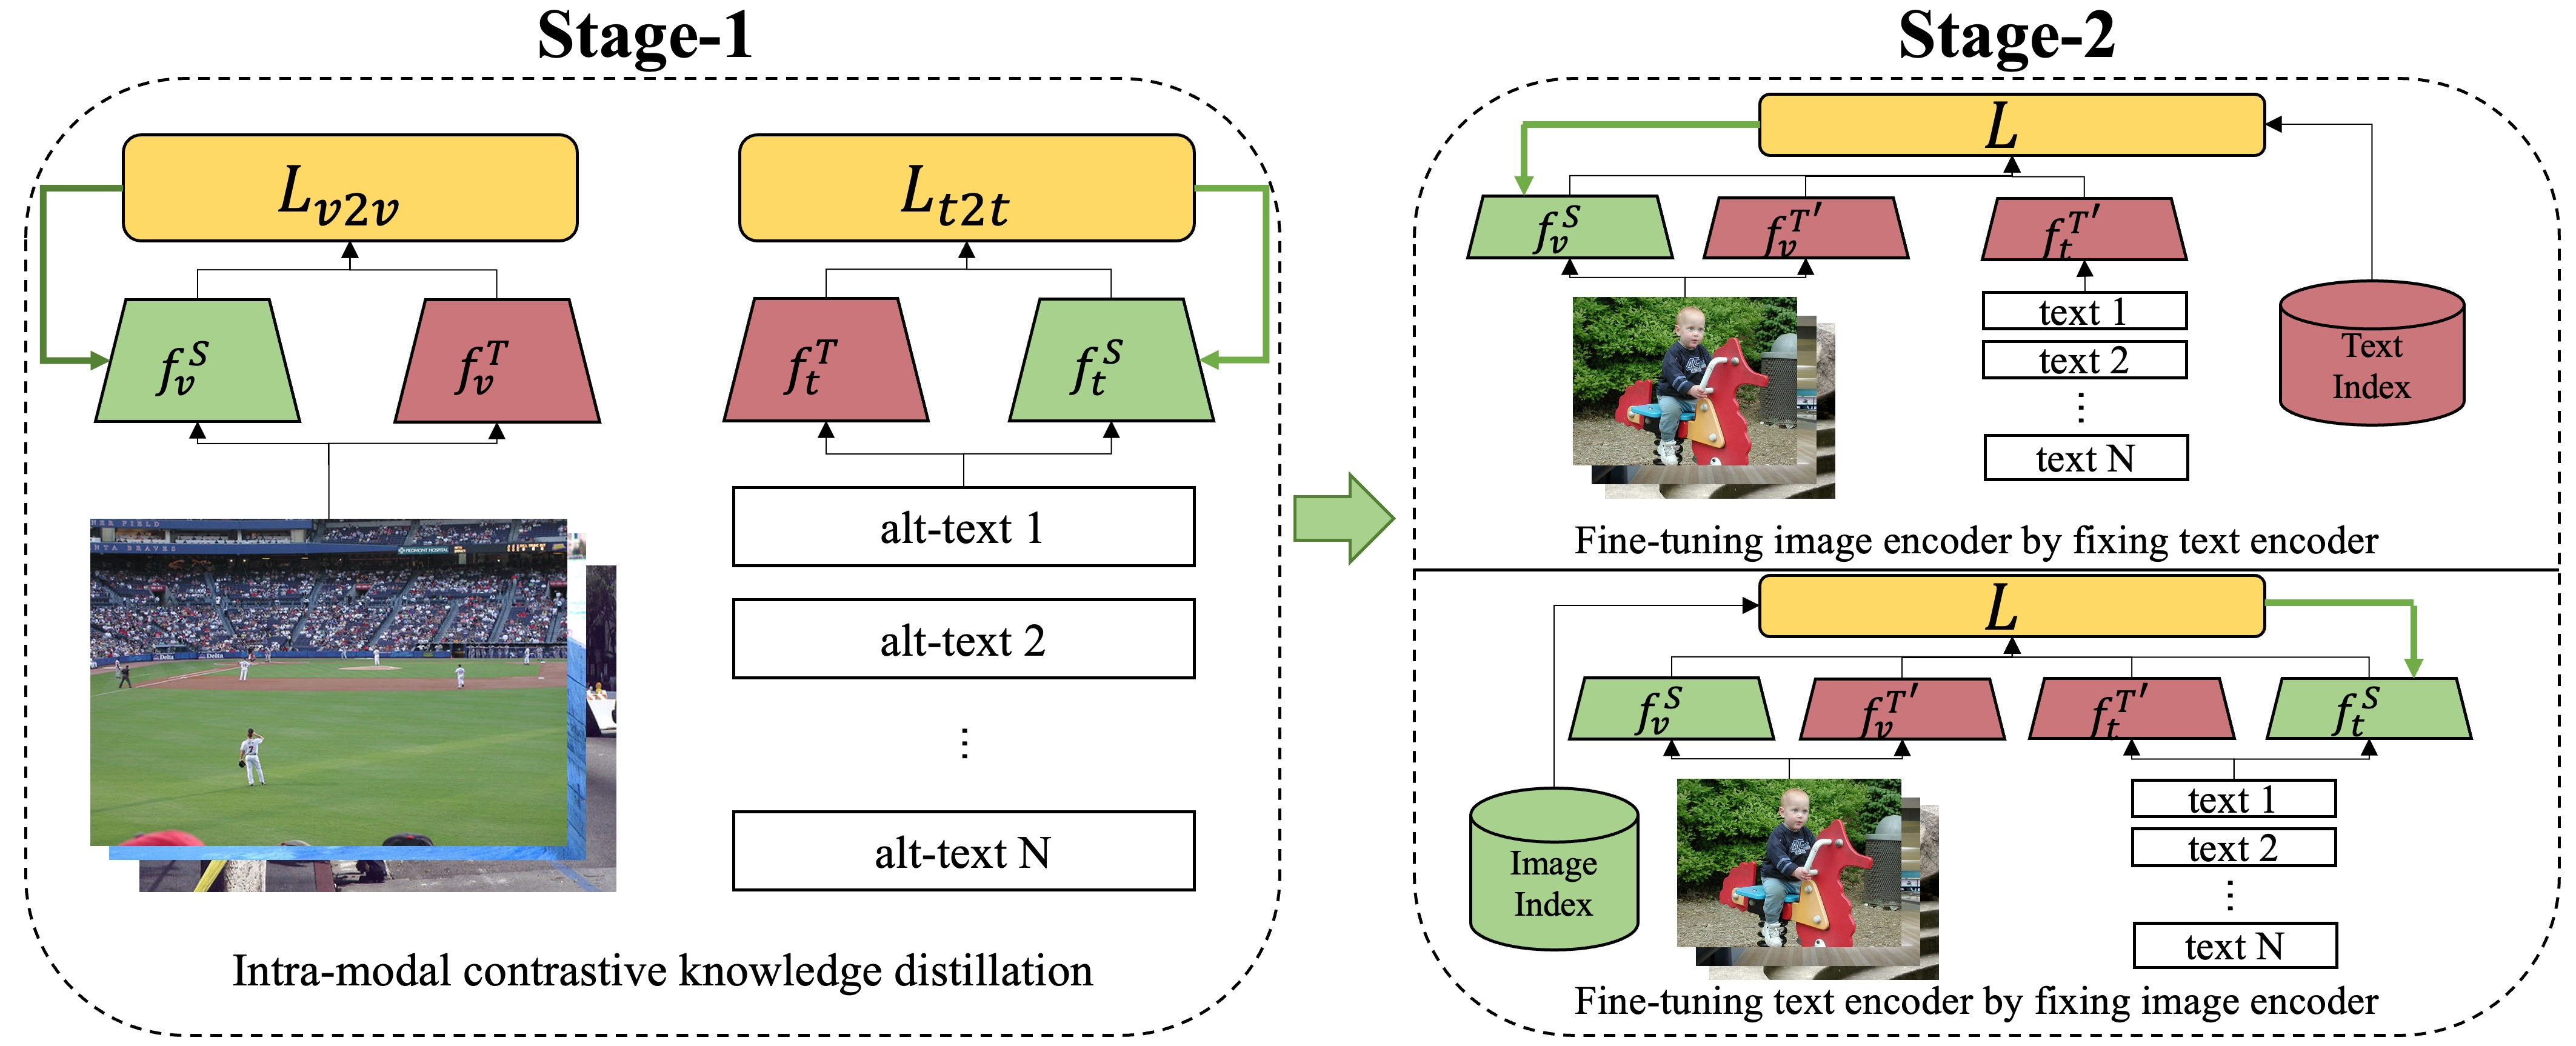
\includegraphics[width=2.0\columnwidth]{figures/retrieval.png}}
	\caption{In stage-1~(\secref{stage1}), we perform  \textit{intra-modal} contrastive knowledge distillation. In stage-2~(\secref{stage2}), we sequentially fine-tune  $f_v^{S}$ and $f_t^{S}$ with knowledge distillation~(KD) and corpus-level hard negative~(HN) mining via pre-computed index. The total loss $L$ is the sum of $L_{t2v}$, $L_{v2t}$, $L_{KD}$, and $L_{HN}$. The thin black arrows represent the input/output flows and 
the solid green arrows indicate the gradient flows.
		%\KZ{Many of the symbols are not introduced at this stage. So
		%either make the annotations more explicit, or explain the notations in the caption.
		%Also label the key process such as distillation and what stage-1 and stage-2 each
		%does in the pic.
		%Make the figure self-explanatory without having the look at the main text.}
	} \label{fig:overview}
\end{figure*}

However, a more practical scenario calls for dynamic indexing of new images into the pool,
which requires both the image encoder and the text encoder to be resident in memory. 
This makes the above approach less practical on mobile devices which have limited
memory and processing power. Unfortunately, little attention has been paid to fulfill this need. 
%are still memory intensive and computationally expensive considering scenarios where the image encoder also needs to reside constantly in memory to support incremental indexing. 
In this paper, we show that a large dual-encoder model can be compressed into 
a much smaller and faster counterpart while retaining its retrieval accuracy 
using a novel two-stage compression framework. 
In the first stage, we make use of abundant non-paired texts/images to separately 
compress text or image encoder with an effective intra-modal contrastive knowledge 
distillation scheme. In the second stage, we sequentially fine-tune the distilled image or
text encoder on paired text-image data with comprehensive learning objectives.
%\KZ{I think you need to be more specific about the novelty of the approach.
%For example, what has been attempted before (maybe in other context), what is
%really new here?} 
Using CLIP~\cite{clip} as the target model, our compressed models deliver comparable performance on MSCOCO and Flickr30K while being just 39\% of the original size 
and 1.6x/2.9x times faster for processing image/text. 
Detailed ablation study shows the effectiveness of each component in the 
compression framework and their synergistic effects. 

Our contributions are three-folds: 1)~an effective compression framework tailored for lightweight text-image retrieval; 2)~a leaner and faster model with competitive accuracy; 3)~open-sourced models and text-to-image search mobile applications on both iOS and Android at \url{https://anonymous.4open.science/r/MoTIS-B7E5}.
